\documentclass[12pt]{article}

\usepackage{pdfpages}
\usepackage{graphicx}
\usepackage{float}

\title{Project Progress Update}
\author{Ian Ooi}
\date{Due April 15, 2014}

\begin{document}
    \maketitle
    \section{Overview}
        The video shows a piece of paper that folds itself into a origami crane then flies off.  Produced with stop motion, the video requires that supports and wires be used to hold the paper in position for capture of the frame.  To remove the supports in each frame to make the paper appear to be folding itself, a combination of inpainting, matting, and poisson editing was used.  The original plan involved the crane flying outside, but the current state of the video does not include this sequence.  
        %\subsection{Storyboard}
        %    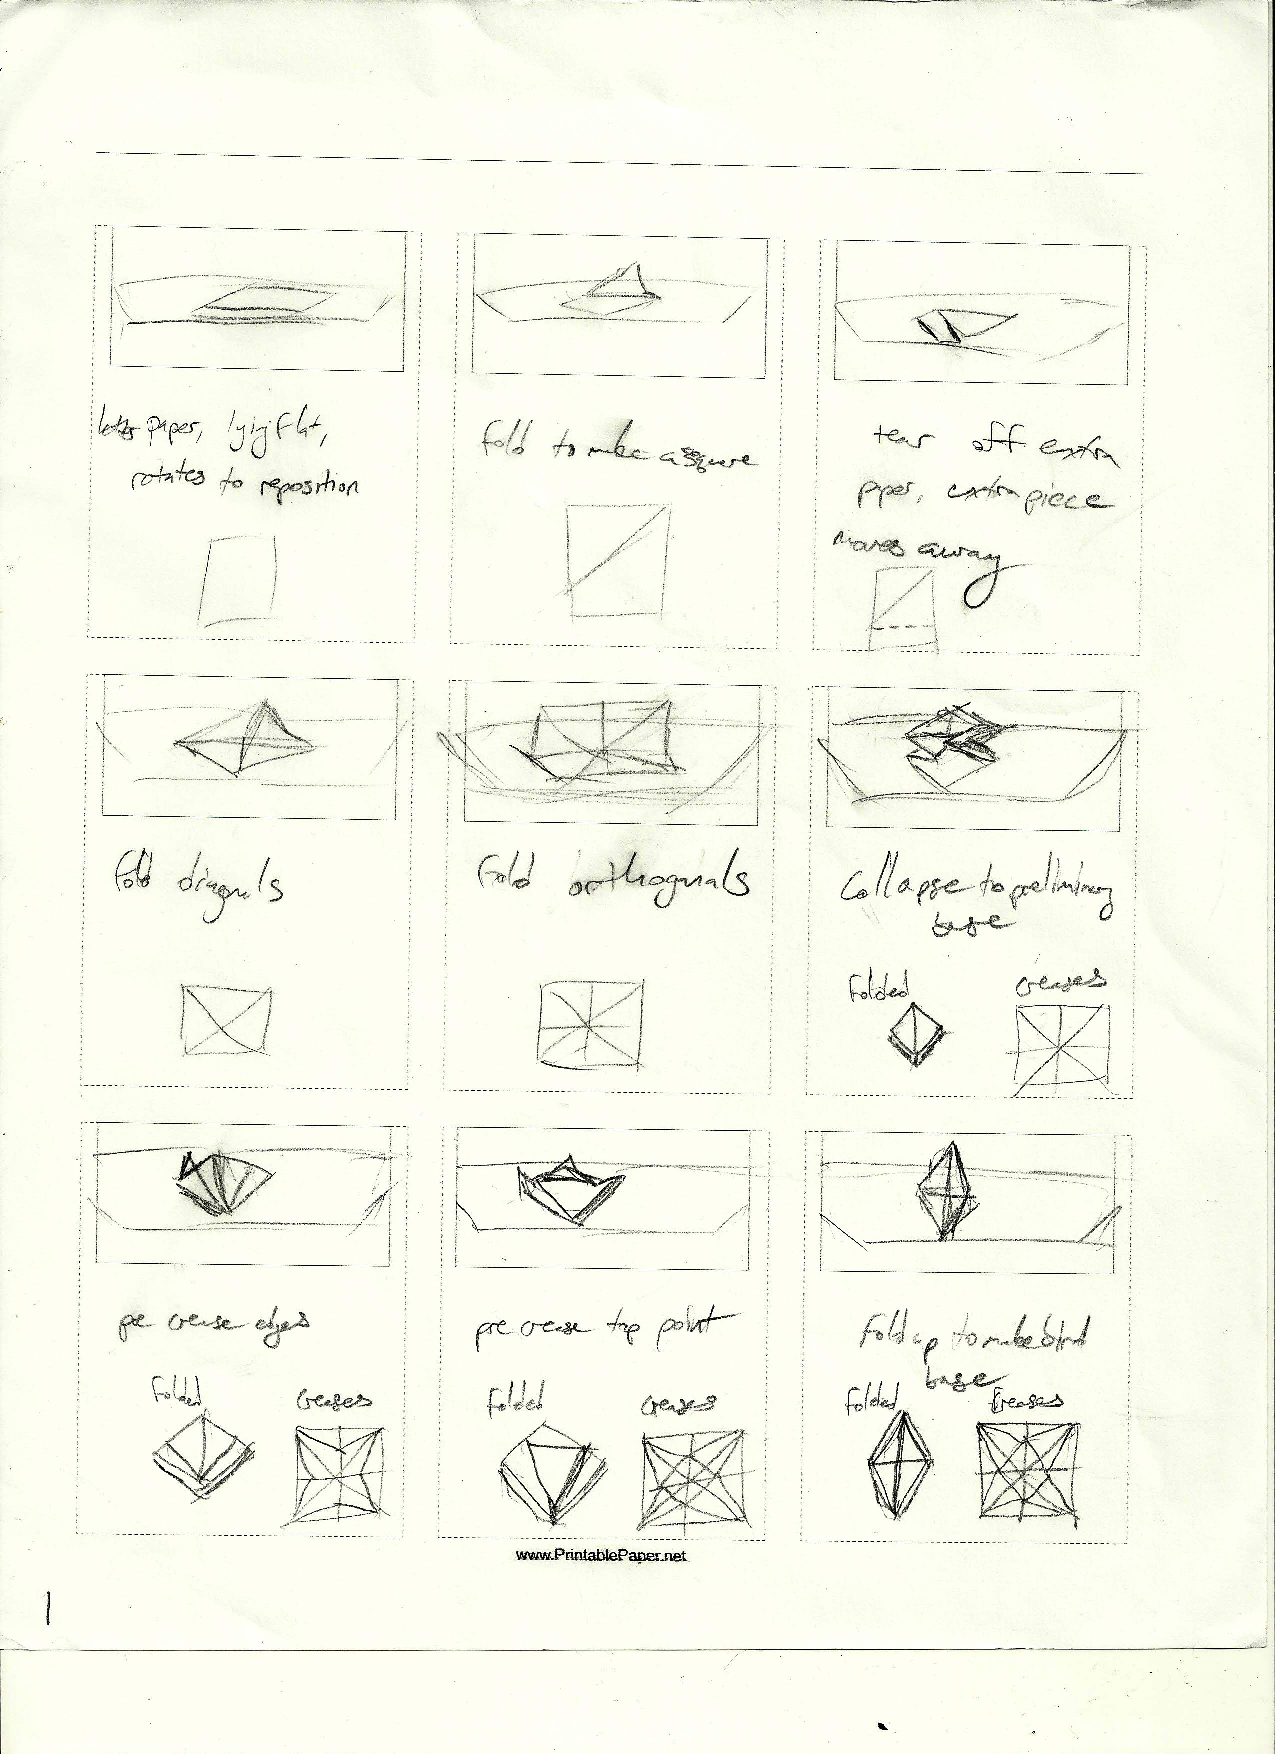
\includepdf[pages={1,2,3}]{storyboard.pdf}
    \section{Related Work}
        Stop motion is a style chosen for its aesthetics and production style.  Films such as Coraline, Paranorman, Wallace and Gromit, Chicken Run, the Corpse Bride, and the shorts by PES such as Fresh Guacamole.  Low cost and improved detail and texture are both factors in the choice to use stop motion, in addition to the distinctive style.  The relative ease of production, subject matter (origami is fairly conducive to stop motion as it is static, positionable, and somewhat rigid in its movements), and cleanliness of the frames (i.e. no motion blur or similar effects) contributed to the choice of stop motion.
        
        Inpainting and compositing are commonly used effects in the field of visual effects, and can be used in conjunction with stop motion to remove any wires, stands, and pieces that are used for structure, support and positioning but are not intended for the final cut.  The techniques are described in Computer Vision for Visual Effects by Radke.  Several inpainting techniques were used, including the Navier-Stokes and Telea inpainting methods \cite{ns, telea}.  The resynthesizer plugin in GIMP was also used for clean-up, mostly due to the rich selection tools available in gimp for targeting problem areas one by one.  The claim has been that the resynthesizer plugin uses PatchMatch \cite{patchmatch}, though the official page does not state the algorithm(s) used.

        For extreme cases, where a large portion of the scene is occluded, patches are borrowed from other frames, using a matte.  
        
    \section{Data Collection}
        Data was collected in 4 bursts.  A  camera was set up on a tripod overlooking the scene, which was then posed and photographed to produce the next frame.  The camera was fitted with a 50mm prime lens, and was set with 1/30 shutter speed, f-stop of 13, and ISO 2000.  A dark blue background was used for the folding shots as well as for the flapping wing sequence.  Outdoor scenes are to be collected on the next clear (or somewhat clear) day to attempt to get blue skies.  Around 350 useful frames were collected for the folding sequence, as well as 24 frames for a general flapping sequence (for use in the outdoor sequence).

        Data collection sessions were fairly short considering the frames captured, but when mistakes were made large sections of the sequence would have to be re-shot.
        
    \section{Technical Approach}
        The frames are captured with minimal supports for the model.  Wires are used for propping up and manipulating the model frame to frame, ensuring controlled maneuvers.  A static tripod setup was used to ensure consistency between frames.    

        Once captured, a combination of inpainting, matting, and poisson image editing was used to produce the final frames.  The general case was that there was a wire that could be inpainted, filling in the background and some minor sections of the crane.  This was performed using several passes of inpainting, utilizing a combination of OpenCV's inpainting function and the GIMP resynthesizer plugin.  For most frames, the first pass was with OpenCV's inpainting function, with cleanup done with the GIMP resynthesizer plugin (as this allowed manual selection of problem regions).  

        For extreme cases, such as an arm or large segment of wire showing in a frame, a matte was generated using OpenCV's grabcut implementation.  
        
        %From this setup, it is a simple matter of using image compositing and inpainting to remove wires and stands from the frames.  Some frames were harder to set up, and were captured with manual positioning of the crane (i.e. I was holding it with my hand).  Patchmatch implementations are available in tools such as photoshop, and code implementations can be found for inpainting techniques on the internet.  Image compositing and matting samples can also be found.  The wires used were generally green in color to differentiate from the background used, so a simple detection scheme could be used to find the wires and remove them in a batch edit as opposed to editing each frame.  This would be the final goal.  A tracking system could also be used, but due to the nature of the footage, it shouldn't be required.  For the outdoor sequence, the images should be composited onto the backgrounds, again as a batch.
        
    \section{Sample Frames}
        \subsection{Example Sequence}
            \begin{figure}[H]
                \centering
                \includegraphics[width=0.3\textwidth]{input_frames/IMG_3056.JPG}
                \includegraphics[width=0.3\textwidth]{input_frames/IMG_3057.JPG}
                \includegraphics[width=0.3\textwidth]{input_frames/IMG_3058.JPG}
                \includegraphics[width=0.3\textwidth]{input_frames/IMG_3059.JPG}
                \includegraphics[width=0.3\textwidth]{input_frames/IMG_3060.JPG}
                \caption{Unedited sequence.}
            \end{figure}
            \begin{figure}[H]
                \centering
                \includegraphics[width=0.3\textwidth]{frames/IMG_3056.JPG}
                \includegraphics[width=0.3\textwidth]{frames/IMG_3057.JPG}
                \includegraphics[width=0.3\textwidth]{frames/IMG_3058.JPG}
                \includegraphics[width=0.3\textwidth]{frames/IMG_3059.JPG}
                \includegraphics[width=0.3\textwidth]{frames/IMG_3060.JPG}
                \caption{Edited sequence.}
            \end{figure}
        \subsection{Successes and Ideal Cases}
            \begin{figure}[H]
                \centering
                \includegraphics[width=0.3\textwidth]{input_frames/IMG_3056.JPG}
                \includegraphics[width=0.3\textwidth]{input_frames/IMG_3057.JPG}
                \includegraphics[width=0.3\textwidth]{input_frames/IMG_3058.JPG}
                \includegraphics[width=0.3\textwidth]{input_frames/IMG_3059.JPG}
                \includegraphics[width=0.3\textwidth]{input_frames/IMG_3060.JPG}
                \caption{Unedited sequence.}
            \end{figure}
            \begin{figure}[H]
                \centering
                \includegraphics[width=0.3\textwidth]{frames/IMG_3056.JPG}
                \includegraphics[width=0.3\textwidth]{frames/IMG_3057.JPG}
                \includegraphics[width=0.3\textwidth]{frames/IMG_3058.JPG}
                \includegraphics[width=0.3\textwidth]{frames/IMG_3059.JPG}
                \includegraphics[width=0.3\textwidth]{frames/IMG_3060.JPG}
                \caption{Edited sequence.}
            \end{figure}
            
        \subsection{Failure cases}
        \subsection{Example of combination of effects to produce final frame}
    \section{Future work}
        The original plan involved the crane flying outside, but I spent instead a lot of time getting the indoor sequence to look good with various tweaks.  Ideally the final sequence of the crane flying outside into the sky would be completed and added.  The current video also does not contain the last few frames of flight after the crane is completed, as I ran out of memory during the video creation.  As I was making this I actually thought that it would have been cooler to have started with a picture of a seagull, crane, heron or pigeon and perform a morph from the bird to a crane which then flies inside and unfolds itself, but unfortunately I didn't think of this soon enough.

    \nocite{grabcut}
    \nocite{telea}
    \nocite{ns}
    \nocite{poisson}

    \bibliographystyle{plain}
    \bibliography{refs.bib}
\end{document}
